%!TEX ROOT = thesis.tex
\chapter{IMPLEMENTATION PLAN AND INITIAL RESULTS}
\section{Planning}

An implementation strategy was created with milestones achieve at key project
checkpoints in order to complete the project in a timely manner. In figures \ref{tab:gantt-chart-fyp1} and \ref{tab:gantt-chart-fyp2} , two Gantt charts were created to make it easier to keep
track our progress in FYP 1 and FYP 2.  Table 5.1 and Table 5.2, respectively, contain the detailed description of the milestones displayed in the respective Gantt charts.


\FloatBarrier
\begin{table}[]
\centering
\begin{tabular}{|c|l|l|l|l|l|}
\hline
\textbf{TASK}                                 & \multicolumn{1}{c|}{\textbf{OCT}}             & \multicolumn{1}{c|}{\textbf{NOV}}             & \textbf{DEC}             & \textbf{JAN}             & \textbf{FEB}             \\ \hline
\textit{\textbf{Knowledge Gaining}}           & \multicolumn{1}{c|}{\cellcolor[HTML]{FFCB2F}} & \multicolumn{1}{c|}{\cellcolor[HTML]{FFCB2F}} & \cellcolor[HTML]{FFCB2F} & \cellcolor[HTML]{FFCB2F} & \cellcolor[HTML]{FFCB2F} \\ \hline
\textit{\textbf{Literature Review}}           & \multicolumn{1}{c|}{\cellcolor[HTML]{FFCB2F}} & \multicolumn{1}{c|}{\cellcolor[HTML]{FFCB2F}} & \cellcolor[HTML]{FFCB2F} &                          &                          \\ \hline
\textit{\textbf{Data Collection}}             & \multicolumn{1}{c|}{}                         & \multicolumn{1}{c|}{\cellcolor[HTML]{FFCB2F}} & \cellcolor[HTML]{FFCB2F} &                          &                          \\ \hline
\textit{\textbf{Data Pre-processing}}         & \multicolumn{1}{c|}{}                         & \multicolumn{1}{c|}{\cellcolor[HTML]{FFCB2F}} & \cellcolor[HTML]{FFCB2F} &                          &                          \\ \hline
\textit{\textbf{Model Searching}}             &                                               & \cellcolor[HTML]{FFCB2F}                      & \cellcolor[HTML]{FFCB2F} &                          &                          \\ \hline
\textit{\textbf{Model Testing}}               &                                               &                                               & \cellcolor[HTML]{FFCB2F} & \cellcolor[HTML]{FFCB2F} &                          \\ \hline
\textit{\textbf{Model Design}}                &                                               &                                               & \cellcolor[HTML]{FFCB2F} & \cellcolor[HTML]{FFCB2F} &                          \\ \hline
\textit{\textbf{Model Implementation}}        &                                               &                                               & \cellcolor[HTML]{FFCB2F} & \cellcolor[HTML]{FFCB2F} &                          \\ \hline
\textit{\textbf{Preliminary Result Analysis}} &                                               &                                               &                          & \cellcolor[HTML]{FFCB2F} & \cellcolor[HTML]{FFCB2F} \\ \hline
\textit{\textbf{Report Writing}}              & \cellcolor[HTML]{FFCB2F}                      & \cellcolor[HTML]{FFCB2F}                      & \cellcolor[HTML]{FFCB2F} & \cellcolor[HTML]{FFCB2F} & \cellcolor[HTML]{FFCB2F} \\ \hline
\textit{\textbf{FYP 1 Presentation}}          &                                               &                                               &                          &                          & \cellcolor[HTML]{FFCB2F} \\ \hline
\end{tabular}
\caption{Gantt Chart for FYP 1}
\label{tab:gantt-chart-fyp1}
\end{table}

\begin{table}[]
\begin{tabular}{|l|l|}
\hline
\multicolumn{1}{|c|}{\textbf{Task}}                       & \multicolumn{1}{c|}{\textit{\textbf{Description}}}                                                                                                                                                                                                                                   \\ \hline
\textit{\textbf{Knowledge Gaining}} & \begin{tabular}[c]{@{}l@{}}Browse and research about the knowledge and\\ information needed for this projects such as\\ fundamental for deep learning, basic operation\\ in Pytorch, use cases of different deep\\ learning models and semantic segmentation technique.\end{tabular} \\ \hline
\textit{\textbf{Literature Review}}                       & \begin{tabular}[c]{@{}l@{}}Perform background study for relevant\\ approaches done by other researcher\end{tabular}                                                                                                                                                                  \\ \hline
\textit{\textbf{Data Collection}}                         & \begin{tabular}[c]{@{}l@{}}Research, collect and download satellite images labelled \\ for semantic segmentation.\end{tabular}                                                                                                                                                       \\ \hline
\textit{\textbf{Data Preprocessing}}                      & Process LoveDA dataset.                                                                                                                                                                                                                                                              \\ \hline
\textit{\textbf{Model Searching}}                         & \begin{tabular}[c]{@{}l@{}}Browse and research different open source\\ models to find out suitable models for this\\ project\end{tabular}                                                                                                                                            \\ \hline
\textit{\textbf{Model Testing}}                           & \begin{tabular}[c]{@{}l@{}}Testing out different selected models to\\ understand the models better and evaluate the\\ results\end{tabular}                                                                                                                                           \\ \hline
\textit{\textbf{Model Design}}                            & \begin{tabular}[c]{@{}l@{}}Make an initial design  of a semantic segmentation model\\  for satellite images.\end{tabular}                                                                                                                                                            \\ \hline
\textit{\textbf{Model Implementation}}                    & \begin{tabular}[c]{@{}l@{}}Make an initial implementation to corroborate\\ the theory in FYP 1.\end{tabular}                                                                                                                                                                         \\ \hline
\textit{\textbf{Model Evaluation}}                        & \begin{tabular}[c]{@{}l@{}}Evaluate the performance of proposed model for\\ future improvement.\end{tabular}                                                                                                                                                                         \\ \hline
\textit{\textbf{Preliminary Results Analysis}}            & \begin{tabular}[c]{@{}l@{}}Perform different experiments and analyze the\\ result to find out important insights.\end{tabular}                                                                                                                                                       \\ \hline
\textit{\textbf{Report Writings}}                         & \begin{tabular}[c]{@{}l@{}}Write up the introduction, background study,\\ proposed method and some analysis in FYP1.\end{tabular}                                                                                                                                                    \\ \hline
\textit{\textbf{FYP1 Presentation}}                       & \begin{tabular}[c]{@{}l@{}}Present and explains work done and findings to\\ the supervisor and moderator.\end{tabular}                                                                                                                                                               \\ \hline
\end{tabular}
\caption{Task Description for FYP 1}
\label{tab:task-desc-fyp1}
\end{table}


% Please add the following required packages to your document preamble:
% \usepackage[table,xcdraw]{xcolor}
% If you use beamer only pass "xcolor=table" option, i.e. \documentclass[xcolor=table]{beamer}
\begin{table}[]
\begin{tabular}{|c|l|l|l|l|}
\hline
\textbf{TASK}                                  & \multicolumn{1}{c|}{\textbf{MARCH}}           & \multicolumn{1}{c|}{\textbf{APRIL}}           & \textbf{MAY}             & \textbf{JUNE}            \\ \hline
\textit{\textbf{Knowledge Gaining}}            & \multicolumn{1}{c|}{\cellcolor[HTML]{FFCB2F}} & \multicolumn{1}{c|}{\cellcolor[HTML]{FFCB2F}} & \cellcolor[HTML]{FFCB2F} & \cellcolor[HTML]{FFFFFF} \\ \hline
\textit{\textbf{Model Design}}                 & \cellcolor[HTML]{FFCB2F}                      & \cellcolor[HTML]{FFCB2F}                      & \cellcolor[HTML]{FFFFFF} & \cellcolor[HTML]{FFFFFF} \\ \hline
\textit{\textbf{Model Implementation}}         & \cellcolor[HTML]{FFCB2F}                      & \cellcolor[HTML]{FFCB2F}                      & \cellcolor[HTML]{FFFFFF} & \cellcolor[HTML]{FFFFFF} \\ \hline
\textit{\textbf{Model Evaluation}}             &                                               & \cellcolor[HTML]{FFFFFF}                      & \cellcolor[HTML]{FFCB2F} & \cellcolor[HTML]{FFCB2F} \\ \hline
\textit{\textbf{Model Refinement}}             &                                               & \cellcolor[HTML]{FFFFFF}                      & \cellcolor[HTML]{FFCB2F} & \cellcolor[HTML]{FFCB2F} \\ \hline
\textit{\textbf{Experimental Result Analysis}} &                                               & \cellcolor[HTML]{FFFFFF}                      & \cellcolor[HTML]{FFCB2F} & \cellcolor[HTML]{FFCB2F} \\ \hline
\textit{\textbf{Report Writing}}               & \cellcolor[HTML]{FFCB2F}                      & \cellcolor[HTML]{FFCB2F}                      & \cellcolor[HTML]{FFCB2F} & \cellcolor[HTML]{FFCB2F} \\ \hline
\textit{\textbf{FYP 2 Presentation}}           &                                               &                                               &                          & \cellcolor[HTML]{FFCB2F} \\ \hline
\end{tabular}
\caption{Gantt Chart for FYP 2}
\label{tab:gantt-chart-fyp2}
\end{table}

\begin{table}[]
\begin{tabular}{|l|l|}
\hline
\multicolumn{1}{|c|}{\textbf{Task}}             & \multicolumn{1}{c|}{\textit{\textbf{Description}}}                                                                                                                                                 \\ \hline
\textit{\textbf{Knowledge Gaining}} & \begin{tabular}[c]{@{}l@{}}Browse and research about the knowledge and\\ information needed for this projects such as\\ fundamental for deep learning, basic operation\\ in Pytorch, use cases of different deep\\ learning models and semantic segmentation technique.\end{tabular} \\ \hline

\textit{\textbf{Model Design}}                  & \begin{tabular}[c]{@{}l@{}}Make a final design  of a semantic segmentation model\\  for satellite images.\end{tabular}                                                                             \\ \hline
\textit{\textbf{Model Implementation}}          & Implement the final model.                                                                                                                                                                         \\ \hline
\textit{\textbf{Model Evaluation}}              & \begin{tabular}[c]{@{}l@{}}Evaluate the performance of proposed model for\\ future improvement.\end{tabular}                                                                                       \\ \hline
\textit{\textbf{Model Refinement}}              & \begin{tabular}[c]{@{}l@{}}Refine the proposed model by doing some\\ slight modification tp the architecture and\\ hyperparameters of model to improve the\\ performance of the model\end{tabular} \\ \hline
\textit{\textbf{Experimental Results Analysis}} & \begin{tabular}[c]{@{}l@{}}Perform different experiments and analyze the\\ result to find out important insights.\end{tabular}                                                                     \\ \hline
\textit{\textbf{Report Writing}}                & \begin{tabular}[c]{@{}l@{}}Write up the introduction, background study,\\ proposed method and some analysis in FYP2.\end{tabular}                                                                  \\ \hline
\textit{\textbf{FYP2 Presentation}}             & \begin{tabular}[c]{@{}l@{}}Present and explains work done and findings to\\ the supervisor and moderator.\end{tabular}                                                                             \\ \hline
\end{tabular}
\caption{Task Description for FYP 2}
\label{tab:task-desc-fyp2}
\end{table}

\FloatBarrier

\section{Initial Results}

The summary of the result of our experiments is shown in Figure \ref{tab:result}. For our U-Net model that was used to provide the baseline performance achieved an mIoU of 33.6\%. It took 4.5 hours to train the U-Net model and it has 2.4 million parameters. 

Our UNetFormer model gave an mIoU of 72.5\% which is a very significant increase compared to U-Net. However it took 14.2 hours to train the UNetFormer model and the model has 11.2 million parameters. The model size and training time is a huge concern and it would be our main objective in FYP 2 to reduce its size and training time. 
\FloatBarrier
\begin{table}[!h]
\centering
\begin{tabular}{|c|c|c|c|}
\hline
\textbf{Model}      & \textbf{mIoU} & \textbf{Parameters} & \textbf{Training Time} \\ \hline
\textbf{U-Net}      & 33.6          & 2.4 M               & 4.5 hours              \\ \hline
\textbf{UNetFormer} & 72.5          & 11.2 M              & 14.2 hours             \\ \hline
\end{tabular}
\caption{Baseline and Initial Result}
\label{tab:result}
\end{table}
\FloatBarrier

Figure \ref{fig:train} is a sample image from the testing dataset and \ref{fig:result} displays the segmentation result from U-Net and UNetFormer. We observed that U-Net struggles to classify that are within the boundary of pixels from another class. It also struggles to classify large objects that span across the image. On top of that, the edges between the classes are not very sharp. Compared its result to UNetFormer, the edges produced are very sharp and it has little problems of classifying small objects that are surrounded by other large objects.
\FloatBarrier
\begin{figure}[!h]
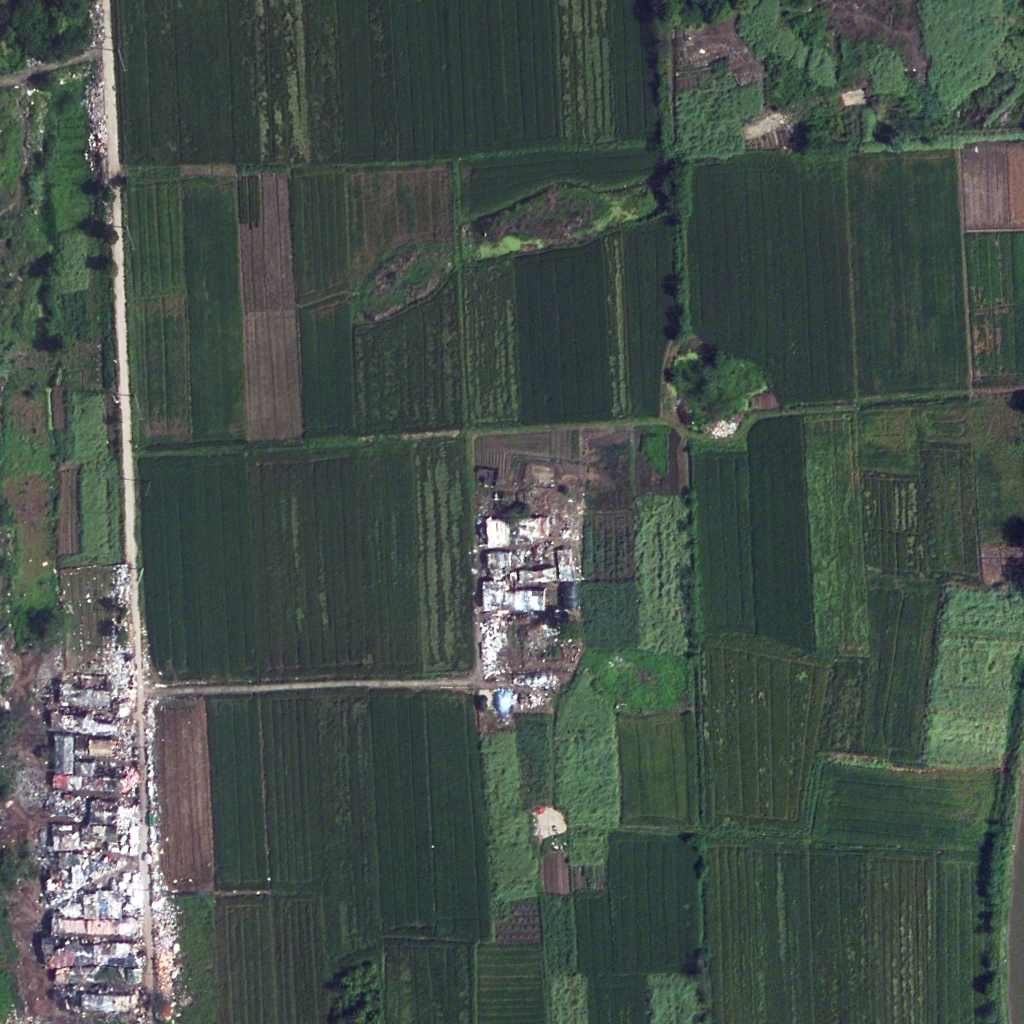
\includegraphics[width=9.5cm, height=6.5cm]{images/3592.png}
\centering
\caption{An Image From The Test Set}
\label{fig:train}
\end{figure}

\begin{figure}[!htb]
    \centering
    \begin{minipage}{0.5\textwidth}
        \centering
        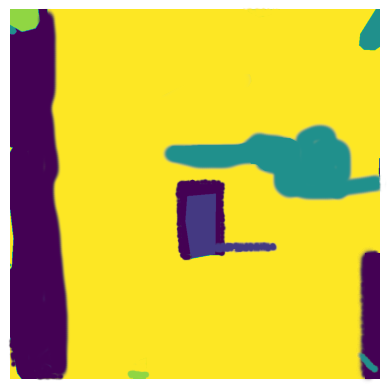
\includegraphics[width=0.95\textwidth, height=0.35\textheight]{images/3592-unet.png}
    \end{minipage}\hfill
    \begin{minipage}{0.5\textwidth}
        \centering
        
\includegraphics[width=0.95\textwidth, height=0.35\textheight]{images/3592-unetformer.png}
    \end{minipage}
\caption{(a) Segmentation Result From U-Net (b) Segmentation Result from UNetFormer}
\label{fig:result}
\end{figure}
\FloatBarrier

